% Load the base class
\documentclass[minted, draw]{../tex/hebdomon}
\usepackage{svg}

\newif\ifshowcode
\showcodefalse % or \showcodetrue

\usepackage[T1]{fontenc}
\usepackage[utf8]{inputenc} % se usi PDFLaTeX
\begin{document}

\title{Blood Cells Detection and Classification using Deep Learning and Machine Learning}
\author{v0.1}
\StudentName{Achille Cannavale}
\date{dtm@mci4me.at}



\begin{titlepage}
    \centering
	
\includegraphics[width=4cm]{figures/logo.png}\par\vspace{1cm}

    %\vspace*{2cm}

    {\scshape\LARGE Università degli Studi di Cassino e del Lazio Meridionale\par}
    \vspace{1cm}
    {\Large Corso di Laurea Magistrale in Ingegneria Informatica \par}

    \vspace{2cm}
    {\Huge\bfseries Blood Cells Detection and Classification using Deep Learning and Machine Learning\par}
    \vspace{1cm}
    {\large Versione 0.1}

    \vfill

    \begin{flushleft}
    \textbf{Cannavale Achille} \\
    \textbf{Colacicco Nunziamaria} \\
    \textbf{La Torre Noemi} \\
    \end{flushleft}

    \vspace{1.5cm}

    {\large \today\par}
\end{titlepage}

\dominitoc
\tableofcontents
\newpage

\Chapter{}
\Section{Introduzione}

La malaria è una delle principali malattie infettive a livello globale, con un impatto significativo sulla salute pubblica, in particolare nei paesi tropicali e subtropicali. Tra i diversi parassiti responsabili di questa patologia, il \hlight{Plasmodium vivax} rappresenta una delle specie più diffuse. La diagnosi precoce e accurata è fondamentale per un trattamento tempestivo ed efficace, e l’analisi microscopica degli strisci ematici rimane uno degli strumenti diagnostici più affidabili.
In questo progetto, viene affrontato il problema della rilevazione e classificazione automatica delle cellule del sangue infettate da P. vivax, attraverso tecniche di machine e deep learning.
Utilizzando il dataset \hlight{P. vivax malaria infected human blood smears}, che contiene oltre \textbf{1.300} immagini microscopiche annotate con più di \textbf{86.000} cellule identificate e classificate, si propone una pipeline [FOTO] che combina \textbf{Deep Learning} e \textbf{Machine Learning} per:

\begin{itemize}
	\item individuare automaticamente le regioni di interesse (ROI) contenenti cellule
	\item estrarre le feature significative dalle ROI
	\item classificare ogni cellula in una delle categorie predefinite, tra cui cellule sane (red blood cell e leukocyte) e diversi stadi del parassita infetto (trophozoite, ring, gametocyte, schizont)
\end{itemize}

\begin{warning}
	L’analisi di questo lavoro ha evidenziato una marcata sbilanciatura del dataset, aspetto che ha richiesto un’attenta progettazione delle strategie di addestramento.
\end{warning}
%
\begin{figure}[ht]
	\centering
	\includesvg[width=\linewidth]{figures/pipeline_general.svg}
	\caption{Pipeline Generale del nostro progetto, suddivisa in una fase di Deep Learning per per la rilevazione delle ROI e l'estrazione delle features e una fase di Machine Learning per la classificazione delle cellule.}
\end{figure}
%

\Section{Strumenti utilizzati}

Per lo sviluppo del progetto sono stati adottati diversi strumenti software, suddivisi in base alle funzionalità specifiche per il \textit{deep learning}, il \textit{machine learning} e l’analisi dei dati. La scelta di ciascuno di essi è stata guidata da criteri di efficienza, semplicità d’uso e ampia diffusione nella comunità scientifica.

\begin{itemize}
    \item \textbf{Deep Learning:} \textit{PyTorch} \\
    Utilizzato per la progettazione, l’addestramento e la valutazione dei modelli di deep learning. PyTorch si distingue per la sua flessibilità e l’approccio dinamico alla costruzione delle reti neurali, risultando particolarmente adatto per attività di ricerca e prototipazione rapida.

    \item \textbf{Machine Learning:} \textit{Scikit-learn} \\
    Impiegato per l’implementazione di algoritmi di machine learning tradizionali, grazie alla sua vasta collezione di modelli predefiniti e strumenti per la valutazione delle prestazioni.

    \item \textbf{Strumenti Ausiliari:}
    \begin{itemize}
        \item \textit{NumPy} e \textit{Pandas}: utilizzati per la manipolazione, la pulizia e l’analisi dei dati, fondamentali nella fase di preprocessing e gestione dei dataset.
        \item \textit{Matplotlib}: utilizzata per la visualizzazione grafica dei risultati, utile per l’analisi esplorativa e la presentazione delle performance dei modelli.
    \end{itemize}
\end{itemize}

\Section{Composizione Dataset}

Il dataset utilizzato per questo progetto è composto da \textbf{1.328 immagini} contenenti in totale \textbf{86.035 oggetti annotati}. Ogni oggetto rappresenta una singola cellula o elemento biologico rilevato nelle immagini microscopiche, ed è associato a una delle seguenti \textbf{sette classi}:

\begin{itemize}
    \item \texttt{red blood cell} (83.034)
    \item \texttt{trophozoite} (1.584)
    \item \texttt{ring} (522)
    \item \texttt{difficult} (446)
    \item \texttt{schizont} (190)
    \item \texttt{gametocyte} (156)
    \item \texttt{leukocyte} (103)
\end{itemize}

Come si può osservare dalla distribuzione, il dataset presenta un \textbf{forte sbilanciamento tra le classi}, con la stragrande maggioranza degli oggetti appartenenti alla categoria \texttt{red blood cell}, che rappresenta da sola circa il \textbf{96{,}5\%} del totale.

Questo sbilanciamento costituisce una \textbf{sfida rilevante per i modelli di classificazione}, in quanto tende a favorire la previsione della classe dominante a discapito delle classi minoritarie, che possono essere trascurate o predette con bassa accuratezza.

Per affrontare questo problema, durante lo sviluppo sono state considerate diverse strategie, tra cui:
\begin{itemize}
   \item il bilanciamento del dataset,
   \item l’uso di tecniche di \textit{data augmentation},
   \item l’assegnazione di pesi differenti alle classi durante l’addestramento,
   \item e l’adozione di metriche di valutazione più robuste rispetto alla sola accuratezza, come \textit{precision}, \textit{recall} e \textit{F1-score}.
\end{itemize}


\Chapter{Deep Learning}

\Section{Trasformazioni}
Per garantire una buona generalizzazione del modello, e ridurre l'overfitting, è stata utilizzata la tecnica di \textit{data augmentation} tramite la libreria \texttt{Albumentations}. Dopo una fase di sperimentazione, sono state selezionate le seguenti trasformazioni come le più efficaci per il nostro caso di studio:

%
\begin{table}[H]
	\begin{NiceTabular}{rX}[rules/color=[gray]{0.9},rules/width=1pt]
		\CodeBefore
		\rowcolors{1}{black!5}{}
		\rowcolors{3}{blue!5}{}
		\Body
		\toprule
		\textbf{Trasformazione}      & \textbf{Parametri}                                \\
		\midrule
		\textbf{A.HorizontalFlip} & p=0.5          \\
		\textbf{A.VerticalFlip}   & p=0.5        \\
		\textbf{A.ColorJitter} & brightness=0.2, contrast=0.2, saturation=0.2, hue=0.1, p=0.3\\
		\textbf{A.RandomBrightnessContrast} & p=0.3\\
		\textbf{A.MotionBlur} & p=0.2\\
		\textbf{A.GaussNoise} & p=0.2\\
		\textbf{A.CLAHE} & p=0.2 \\
		\textbf{A.CoarseDropout} & num holes ange=(3, 6), hole height range=(10, 20), hole width range=(10, 20), fill="random uniform", p=0.2 \\
		\textbf{A.Resize} & 800x800 \\
		\textbf{A.Normalize} & mean=[0.7205, 0.7203, 0.7649], std=[0.2195, 0.2277, 0.1588] \\
		\bottomrule
	\end{NiceTabular}
	\caption{Lista delle trasformazioni utilizzate per il dataset.}
\end{table}
%

In particolare, I parametri della normalizzazione sono stati calcolati dal dataset stesso:
\begin{table}[!ht]
	\begin{NiceTabular}{rX}[rules/color=[gray]{0.9},rules/width=1pt]
		\CodeBefore
		\rowcolors{1}{black!5}{}
		\rowcolors{3}{blue!5}{}
		\Body
		\toprule
		\textbf{Parametro}      & \textbf{Valore}                                \\
		\midrule
		\textbf{Media RGB} & (0.7205, 0.7203, 0.7649) \\
		\textbf{Deviazione standard RGB} & (0.2195, 0.2277, 0.1588) \\
		\bottomrule
	\end{NiceTabular}
	\caption{Valori di media e deviazione standard per la normalizzazione delle immagini.}
\end{table}



Una delle trasformazioni che ha avuto il maggiore impatto sulle prestazioni è stata la \texttt{CoarseDropout} (fig. \ref{fig:coarse_dropout_example}), che oscura regioni rettangolari casuali dell’immagine, simulando occlusioni ottiche e migliorando la robustezza del modello in scenari reali dove gli oggetti potrebbero essere parzialmente visibili.

\ifshowcode
\begin{code}{python}
A.CoarseDropout(
    num_holes_range=(3, 6),              # Numero casuale di buchi tra 3 e 6
    hole_height_range=(10, 20),          # Altezza dei buchi tra 10 e 20 px
    hole_width_range=(10, 20),           # Larghezza dei buchi tra 10 e 20 px
    fill="random_uniform",               # Riempie i buchi con valori casuali
    p=0.2                               # Probabilità di applicazione 20%
)
\end{code}
\fi

\begin{figure}[H]
	\centering
	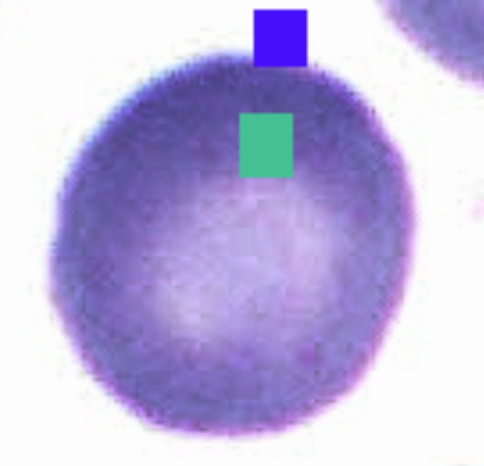
\includegraphics[width=.2\linewidth]{figures/corse_result.png}
	\caption{Esempio di CoarseDropout applicata su una cellula.}
	\label{fig:coarse_dropout_example}
\end{figure}
%


\Section{Personalizzazione delle Anchor Boxes}

Per migliorare le prestazioni del modello di object detection, abbiamo effettuato un’analisi approfondita della distribuzione delle dimensioni delle bounding box presenti nel dataset. Le anchor boxes predefinite, come quelle utilizzate nei dataset generici come COCO, non risultavano ottimali per il nostro caso specifico, in quanto le cellule da rilevare presentano dimensioni e proporzioni piuttosto omogenee e differenti rispetto agli oggetti comuni.

A tal fine, abbiamo estratto tutte le bounding box del dataset di addestramento e calcolato le dimensioni (larghezza e altezza) di ciascuna. I dati così ottenuti sono stati utilizzati come input per un algoritmo di clustering K-Means, impostato per individuare i centroidi rappresentativi delle dimensioni più ricorrenti. In particolare, è stato scelto un numero di cluster pari a 6, corrispondente al numero di anchor boxes da definire. Le nuove ancore suggerite sono state quindi utilizzate per sostituire quelle standard all’interno del modello.

Questa ottimizzazione ha permesso un miglior allineamento tra le proposte del modello e le reali dimensioni degli oggetti nel dataset, contribuendo a un incremento consistente delle metriche di accuratezza. L'impatto dell’adozione delle nuove anchor boxes è illustrato nella Tabella~\ref{tab:custom_anchors}, dove si evidenzia un miglioramento del valore di mAP rispetto alla configurazione predefinita.

\begin{table}[!ht]
	\centering
	\begin{NiceTabular}{rX}[rules/color=[gray]{0.9},rules/width=1pt]
		\CodeBefore
		\rowcolors{1}{black!5}{}
		\rowcolors{3}{blue!5}{}
		\Body
		\toprule
		\textbf{Configurazione Anchor} & \textbf{mAP@0.5} \\
		\midrule
		Default (COCO-style)         & valore \\
		Personalizzate (K-Means)     & \textbf{0.78} \\
		\bottomrule
	\end{NiceTabular}
	\caption{Confronto tra ancore standard e personalizzate.}
	\label{tab:custom_anchors}
\end{table}


\Section{Focal Loss}
Un aspetto cruciale di questo problema è il forte sbilanciamento del dataset: le cellule sane (globuli rossi e leucociti) sono molto più numerose rispetto alle cellule infette, che rappresentano una minoranza spesso difficile da distinguere.

Questo squilibrio comporta che durante l’addestramento i modelli tendano a privilegiare la classificazione corretta delle classi maggioritarie, a discapito di quelle minoritarie, che sono però di massima importanza per una diagnosi accurata e precoce della malaria.

Per mitigare questo problema, abbiamo adottato la \textit{Focal Loss} (Lin et al., 2017), una funzione di perdita che estende la Cross Entropy introducendo un termine di modulazione. Tale termine riduce il peso degli esempi facili (correttamente classificati) e concentra l’apprendimento sugli esempi difficili o mal classificati, tipicamente appartenenti alle classi minoritarie. La formulazione della Focal Loss è:

\[
\text{FL}(p_t) = -\alpha (1 - p_t)^\gamma \log(p_t)
\]

dove \( p_t \) è la probabilità stimata per la classe corretta, \(\alpha\) è un fattore di bilanciamento tra classi e \(\gamma\), detto "focusing parameter", controlla la riduzione del peso degli esempi facili.

Nel nostro caso, i parametri \(\alpha = 0.25\) e \(\gamma = 3.0\) sono stati scelti per ottenere un buon equilibrio tra stabilità e miglioramento delle performance. L’uso della Focal Loss ha permesso di:

\begin{itemize}
    \item ridurre l’impatto degli esempi di sfondo abbondanti,
    \item aumentare la sensibilità verso le cellule infette meno rappresentate,
    \item migliorare la convergenza e la capacità discriminativa del modello.
\end{itemize}

La funzione di perdita per la regressione delle bounding box è stata mantenuta invariata, affidandosi alla \textit{Smooth L1 Loss}, che risulta efficace per la localizzazione precisa delle cellule.

Questa scelta ha avuto un impatto positivo sulle metriche di accuratezza e recall, fondamentali in ambito medico per evitare falsi negativi.


%
\begin{figure}[H]
	\centering
	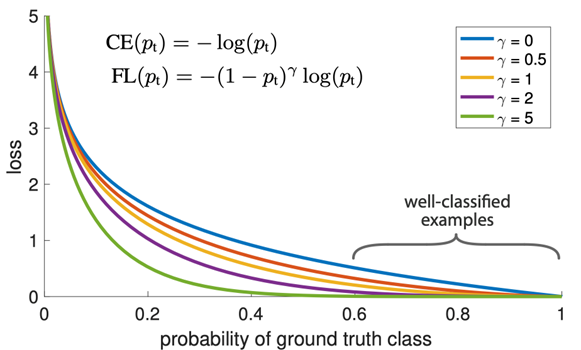
\includegraphics[width=.6\linewidth]{figures/focal_loss.png}
	\caption{Grafico Focal Loss.}
	\label{fig:focal_loss}
\end{figure}
%

\Section{Architetture del Modello}

Durante lo sviluppo del progetto sono state testate diverse architetture di rete neurale, combinando vari \textbf{backbone} con due principali tipologie di \textbf{head}: \hlight{Faster R-CNN} e \hlight{RetinaNet}. L’obiettivo era identificare la combinazione più efficace in termini di accuratezza, capacità di generalizzazione e prestazioni computazionali.

In un modello di object detection, il \textbf{backbone} funge da estrattore di feature: riceve l’immagine in input e produce mappe di caratteristiche utili per individuare e classificare gli oggetti. I backbone testati nel progetto includono:

\begin{itemize}
	\item \hlight{ResNet50}: una rete convoluzionale profonda basata su \hlight{residual blocks}, che permette un’ottima propagazione del gradiente anche in reti molto profonde.
	\item \hlight{ResNet101}: una versione più profonda di ResNet50, che migliora la rappresentazione delle feature a scapito di un maggiore costo computazionale.
	\item \hlight{MobileNet}: una rete più leggera ed efficiente, pensata per dispositivi mobili, ma con performance inferiori in contesti complessi. 
	\item \hlight{ResNeXt101}: un’estensione di ResNet che introduce la dimensione della cardinalità (cioè il numero di percorsi paralleli in ogni blocco), migliorando la capacità di rappresentazione senza aumentare drasticamente i parametri.
\end{itemize}


Il \textbf{detection head}, invece, riceve le feature estratte e produce le predizioni finali (classi e bounding box). Le due architetture di head utilizzate sono:

\begin{itemize}
	\item \hlight{Faster R-CNN}: un approccio a due stadi, in cui un \hlight{Region Proposal Network (RPN)} genera proposte di oggetti che vengono successivamente classificate e regolarizzate. È noto per l’elevata accuratezza, ma è più lento rispetto ad approcci monostadio.
	\item \hlight{RetinaNet}: un metodo \textbf{one-stage} che introduce la \hlight{Focal Loss} per gestire lo squilibrio tra oggetti e background, migliorando le performance su oggetti piccoli o rari. Offre un buon compromesso tra accuratezza e velocità.
\end{itemize}

%
\begin{figure}[H]
  \centering
  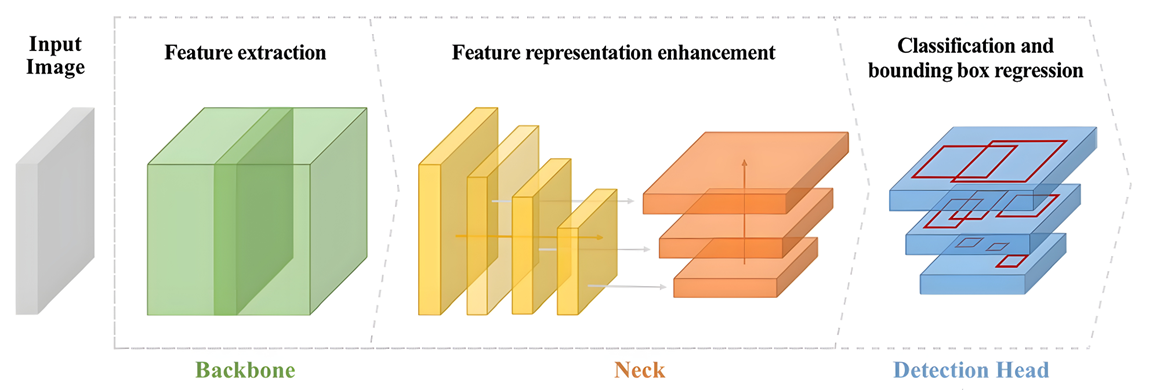
\includegraphics[width=\linewidth]{figures/general_pipeline.png}
  \caption{Pipeline Generale di una rete.}
  \label{fig:general_pipeline}
\end{figure}
%

Le configurazioni testate sono le seguenti:
\begin{itemize}
    \item \textbf{Backbone:} ResNet50 \quad \textbf{Head:} Faster R-CNN
    \item \textbf{Backbone:} ResNet101 \quad \textbf{Head:} Faster R-CNN
    \item \textbf{Backbone:} MobileNet \quad \textbf{Head:} Faster R-CNN
    \item \textbf{Backbone:} ResNet50 \quad \textbf{Head:} RetinaNet
    \item \textbf{Backbone:} ResNeXt101 \quad \textbf{Head:} Faster R-CNN
    \item \textbf{Backbone:} ResNet101 \quad \textbf{Head:} RetinaNet
\end{itemize}

L’architettura che ha fornito i migliori risultati, sia in termini di accuratezza sia di generalizzazione, è stata quella composta da \textbf{ResNeXt101} come backbone e \textbf{Faster R-CNN} come head. In Figura \ref{fig:model_best} è riportata una rappresentazione schematica della pipeline del modello.



%
\begin{figure}[ht]
	\centering
	\includesvg[width=.7\linewidth]{figures/resnext.svg}
	\caption{Pipeline Generale del miglior modello, composto da ResNeXt101 come backbone e Faster R-CNN come head.}
	\label{fig:model_best}
\end{figure}
%

%
\begin{table}[H]
	\begin{NiceTabular}{rX}[rules/color=[gray]{0.9},rules/width=1pt]
		\CodeBefore
		\rowcolors{1}{black!5}{}
		\rowcolors{3}{blue!5}{}
		\Body
		\toprule
		\textbf{Metric}      & \textbf{Value}                                \\
		\midrule
		\textbf{mIoU} & 0.8871 \\
		\textbf{Precision} & 0.9733 \\
		\textbf{Recall} & 0.9683 \\
		\textbf{F1 Score} & 0.9708 \\
		\midrule
		\textbf{mAP} & 0.7397 \\
		\textbf{mAP@50} & 0.9479 \\
		\textbf{mAP@75} & 0.8874 \\
		\bottomrule
	\end{NiceTabular}
	\caption{Evaluation metrics of ResNeXt101 + Faster R-CNN model.}
\end{table}
%

%foto

% Per confronto, è utile visualizzare anche i risultati ottenuti con l’architettura meno performante (MobileNet + Faster R-CNN), mostrati in Figura \ref{fig:model_worst}. Questo confronto evidenzia chiaramente le differenze di accuratezza e qualità della predizione.

%foto

\Section{Valutazione}
\Subsection{Iperparametri}
% Tabella con i parametri
\begin{table}[!ht]
    \begin{NiceTabular}{rX}[rules/color={[gray]{0.9}},rules/width=1pt]
        \CodeBefore
        \rowcolors{1}{black!5}{}
        \rowcolors{3}{blue!5}{}
        \Body
        \toprule
        \textbf{Parameter} & \textbf{Value} \\
        \midrule
        \textbf{BATCH\_SIZE} & 4 \\
        \textbf{NUM\_EPOCHS} & 5 \\
        \textbf{LEARNING\_RATE} & 0.0003 \\
        \textbf{WEIGHT\_DECAY} & 0.001 \\
        \textbf{PATIENCE} & 5 \\
        \textbf{OPTIM} & AdamW \\
        \textbf{SCHEDULER} & ReduceLROnPlateau \\
        \textbf{CustomAnchor} & True \\
        \textbf{loss} & FocalLoss \\
        \textbf{VAL\_SIZE} & 0.2 \\
        \bottomrule
    \end{NiceTabular}
    \caption{Configurazione degli Iperparametri del Miglior Modello.}
    \label{tab:hyperparameters}
\end{table}
%

Gli iperparametri riportati nella Tabella \ref{tab:hyperparameters} sono il risultato di un'attenta fase di sperimentazione in cui sono stati confrontati diversi valori e configurazioni. In particolare, si è osservato che un numero di epoche pari a 5 è sufficiente per ottenere una buona convergenza: aumentare il numero di epoche a 10 non ha portato a miglioramenti significativi in termini di accuratezza o generalizzazione.

Per quanto riguarda l’ottimizzatore, si è confrontato l’uso di Adam e \textbf{AdamW}, con quest’ultimo che ha dimostrato maggiore stabilità e performance migliori, probabilmente grazie alla gestione più efficace della regolarizzazione tramite \textbf{weight decay}.

La politica di gestione del learning rate è stata valutata tra \textbf{ReduceLROnPlateau} e \textbf{CosineAnnealingLR}. \textbf{ReduceLROnPlateau} si è rivelata più adatta al nostro task, poiché riduceva il learning rate solo quando la metrica di validazione non migliorava, consentendo un adattamento più dinamico e mirato rispetto al coseno annealing, che segue un programma fisso.

Infine, la scelta della funzione di perdita si è concentrata tra la \textbf{standard loss} e la \textbf{Focal Loss}. Quest’ultima ha mostrato un vantaggio concreto nella gestione dello sbilanciamento delle classi presenti nel dataset, migliorando la capacità del modello di rilevare correttamente anche le classi meno rappresentate.



\subsection{Visualizzazione dei Risultati}
In questa sezione vengono mostrati i risultati ottenuti dall’addestramento del modello. La Figura \ref{fig:loss_curve} presenta il grafico dell’andamento della \hlight{training loss} e della \hlight{validation loss} durante le epoche, evidenziando una buona convergenza e un’assenza di overfitting significativo.

% Immagine della loss
\begin{figure}[H]
  \centering
  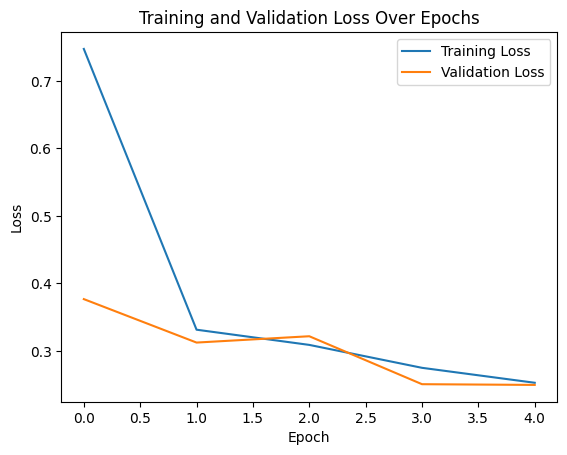
\includegraphics[width=.6\linewidth]{figures/loss.png}
  \caption{Grafico della Training Loss e della Validation Loss.}
  \label{fig:loss_curve}
\end{figure}
%

La Figura \ref{fig:detection_example} mostra un esempio di output del modello su un’immagine del set di test. Le regioni di interesse (ROI) delle cellule sono rappresentate tramite rettangoli di diversi colori: le ROI esatte del dataset sono in \textcolor{teal}{verde}, quelle predette dal modello in \textcolor{red}{rosso}, mentre in \textcolor{blue}{blu} sono evidenziate le cellule non rilevate. Il modello raggiunge un valore medio di \textbf{mIoU} pari a \hlight{0.88}, confermando un’alta precisione nella localizzazione degli oggetti, con un’ottima corrispondenza tra predizioni e annotazioni di riferimento.
% Immagine esempio di un risultato
\begin{figure}[H]
  \centering
  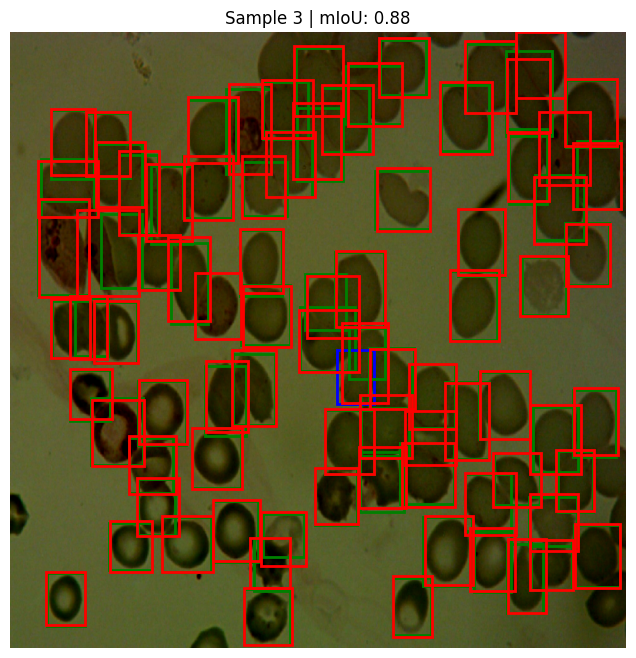
\includegraphics[width=.6\linewidth]{figures/ex_result.png}
  \caption{Risultato di esempio. In rosso sono evidenziate le bounding box correttamente previste dal modello, in blu quelle mancate.}
  \label{fig:detection_example}
\end{figure}
%

\Section{Estrazione delle Feature}
Per l'analisi delle rappresentazioni apprese dal modello, abbiamo implementato una procedura di estrazione delle caratteristiche visive associate alle ROIs predette. Il metodo si basa su un modello di object detection preaddestrato, nello specifico una variante di \textbf{Faster R-CNN con Feature Pyramid Network (FPN)}, che consente di sfruttare rappresentazioni multi-scala per migliorare la localizzazione e classificazione di oggetti di dimensioni variabili.

Durante l'inferenza, ogni immagine del dataset viene elaborata per ottenere le predizioni del modello, comprensive di bounding boxes e punteggi di confidenza. Le predizioni con uno score inferiore a \texttt{score\_threshold} (default: 0.5) vengono scartate. Le restanti predizioni vengono confrontate con i ground truth tramite l'Intersection over Union (IoU), mantenendo solo quelle che superano una soglia di similarità. Questo matching consente di associare ciascuna ROI predetta alla corrispondente annotazione reale.

Le feature vengono estratte dai livelli intermedi del modello tramite la \textbf{backbone con FPN}, che restituisce una gerarchia di mappe di attivazione a risoluzioni diverse. A partire da queste mappe, il modulo \texttt{box\_roi\_pool} seleziona e aggrega le porzioni rilevanti in base alle bounding boxes predette. Le feature pooled vengono poi elaborate dalla \texttt{box\_head}, e ulteriormente arricchite concatenando i \textbf{logit del classificatore} (cls\_score), ottenendo così una rappresentazione congiunta che riflette sia le informazioni visive locali sia le risposte semantiche del modello.


Ogni vettore di feature viene associato a metadati espliciti, tra cui:
\begin{itemize}
	\item l'identificativo dell'immagine
	\item le coordinate della bounding box predetta
	\item il punteggio di confidenza
	\item l’etichetta del ground truth associato
\end{itemize}
 

Tutti i dati raccolti vengono infine aggregati in un dataframe strutturato, che unisce metadati e rappresentazioni numeriche. Il risultato viene salvato in formato CSV per facilitarne l’analisi quantitativa e la visualizzazione.


\Chapter{Machine Learning}

\Section{Introduzione}
%
\begin{figure}[H]
	\centering
	\includesvg[width=\linewidth]{figures/machine_pipeline.drawio.svg}
	\caption{Pipeline generale della parte di Machine Learning.}
\end{figure}
%
La parte di Machine Learning ha come input il file csv generato nella parte di Deep Learning, che contiene le feature estratte dalle ROIs.

In un primo momento, la struttura generale di questa parte era costituita da un solo Classificatore, che aveva il compito di distinguere le cellule in tutte e 7 le classi. Tuttavia, a causa della grande \hlight{class imbalance} del dataset (\ref{fig:sbilanciamento}), si è deciso di adottare un approccio diverso, creando 2 classificatori distinti:
\begin{itemize}
	\item \textbf{Classificatore 1:} \hlight{RBC vs Infected Cells} \\
	Questo classificatore ha il compito di distinguere le cellule sane (RBC e Leukocyte) dalle cellule infette (tutte le altre classi).
	\item \textbf{Classificatore 2:} \hlight{Infected Cells Classification} \\
	Questo classificatore si occupa di distinguere le cellule infette tra loro, classificandole in \texttt{trophozoite}, \texttt{ring}, \texttt{difficult}, \texttt{schizont} e \texttt{gametocyte}
\end{itemize}

% 
\begin{figure}[H]
  \centering
  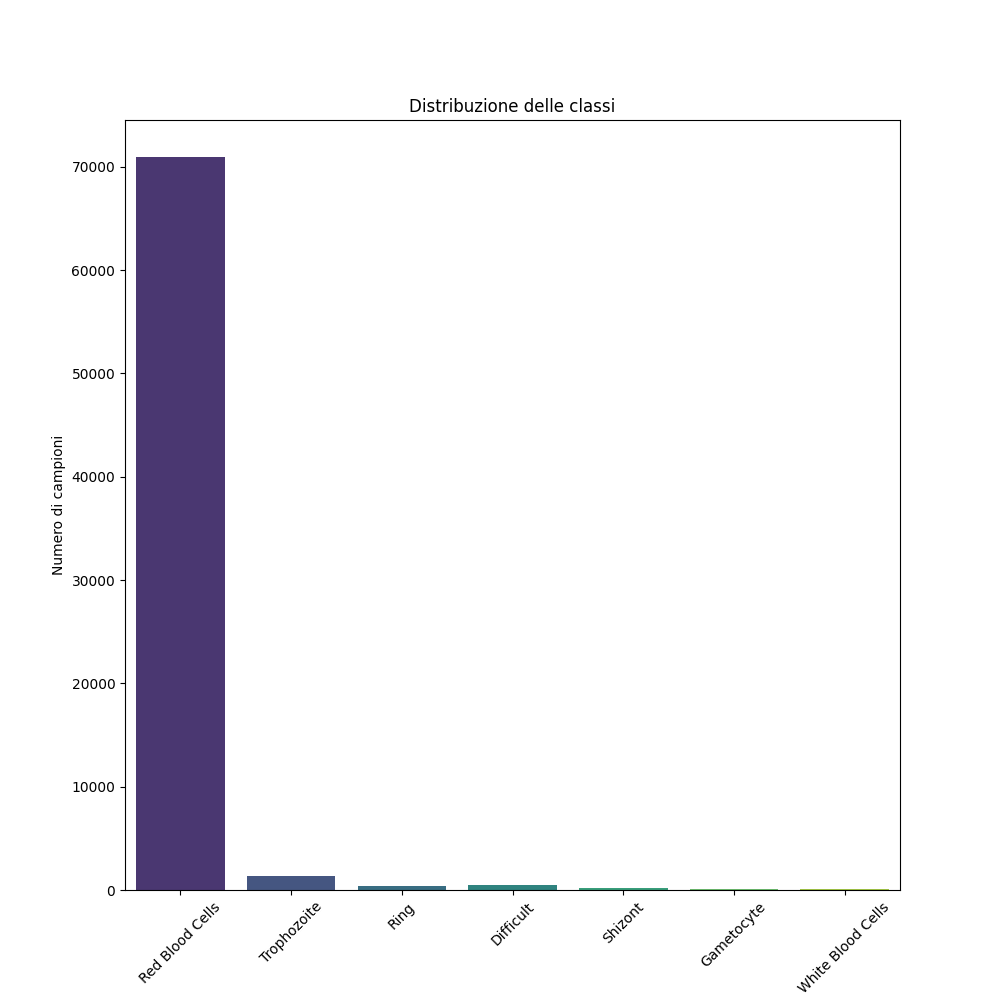
\includegraphics[width=.7\linewidth]{figures/class_distribution.png}
  \caption{Distribuzione delle classi nel dataset prima del preprocessing.}
  \label{fig:sbilanciamento}
\end{figure}
%

\Section{Preparazione del Dataset}
Il dataset non presenta valori mancanti, quindi non è stato necessario effettuare operazioni di \textbf{data cleaning}. Le etichette sono state codificate utilizzando un \textbf{LabelEncoder}, trasformando le classi da etichette testuali o intere non sequenziali in valori numerici consecutivi, come richiesto dalla maggior parte dei modelli di classificazione supervisionata.

\Section{Oversampling: BorderlineSMOTE}
Per affrontare il problema dello sbilanciamento delle classi, è stato utilizzato l'algoritmo \textbf{BorderlineSMOTE}, una variante del Synthetic Minority Over-sampling Technique (SMOTE). Questo metodo genera nuovi campioni sintetici per le classi minoritare, migliorando la capacità del modello di apprendere le caratteristiche distintive delle classi meno rappresentate.
% 
\begin{figure}[H]
  \centering
  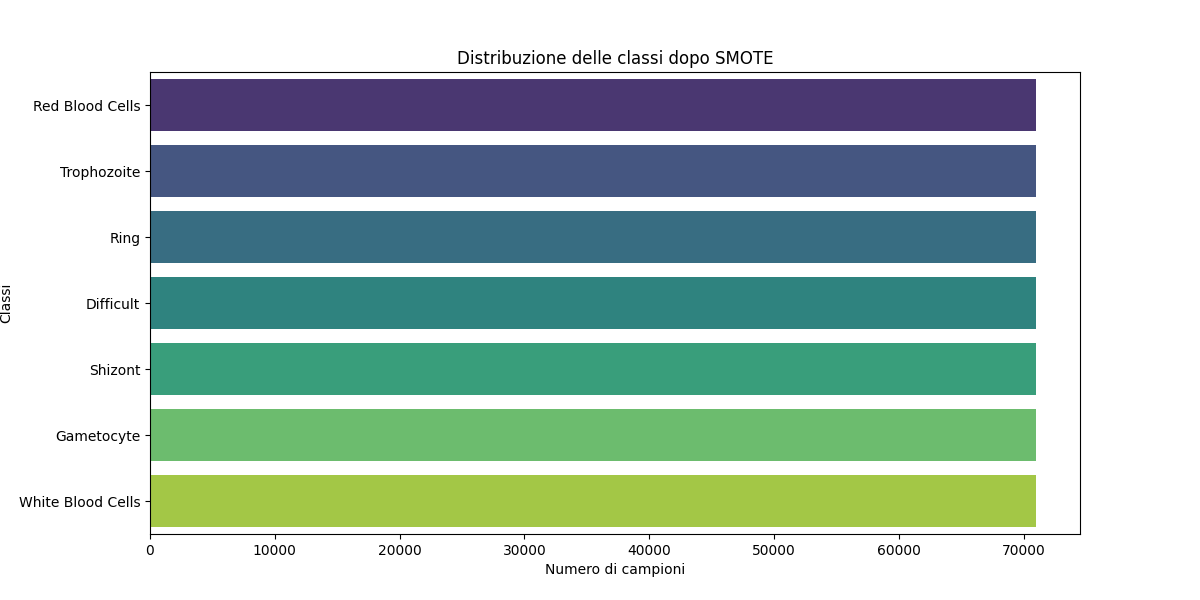
\includegraphics[width=.9\linewidth]{figures/class_distribution_after_smote.png}
  \caption{Distribuzione delle classi nel dataset dopo BorderlineSMOTE.}
  \label{fig:BorderlineSMOTE}
\end{figure}
%

\Section{Variance Threshold}
Per ridurre la dimensionalità del dataset e migliorare le prestazioni del modello, è stata applicata la tecnica di \textbf{Variance Threshold}. Questa tecnica rimuove le feature con una varianza inferiore a una soglia specificata, eliminando le caratteristiche che non apportano informazioni significative. Nel nostro caso, è stata impostata una soglia di 1e-5, portando le features da \hlight{1024 a 767.}

\Section{Normalizzazione}
Poiché le feature presentano range e scale molto differenti, è stata applicata una \textbf{standardizzazione} tramite \textbf{StandardScaler}, che porta ogni variabile ad avere media nulla e deviazione standard unitaria. Questo step è fondamentale per tutti gli algoritmi sensibili alla scala delle feature (come SVM, LDA, KNN), in quanto garantisce pari rilevanza a tutte le variabili numeriche.


\Section{Feature Selection: SelectKBest}
Per contenere la dimensionalità del dataset e ridurre l’overfitting, è stata effettuata una selezione automatica delle feature tramite il metodo \hlight{SelectKBest}, basato su test ANOVA F-test (\texttt{f\_classif}). Questo metodo assegna un punteggio a ogni feature in base alla sua correlazione con la variabile target, selezionando le $k$ migliori.

\Section{Dimensionality Reduction: LDA}
A valle della selezione, è stata applicata anche una tecnica di \textbf{riduzione dimensionale supervisata} tramite \hlight{Linear Discriminant Analysis} (LDA), che proietta i dati in uno spazio a dimensionalità ridotta (fino a $n_{classi} - 1$) massimizzando la separabilità tra le classi. Questo aiuta il modello a concentrarsi solo sulle direzioni rilevanti per la classificazione.

LDA si basa su un principio statistico: cerca di massimizzare il rapporto tra la \textbf{varianza inter-classe} e la \textbf{varianza intra-classe}. Formalmente, l'obiettivo è trovare una proiezione $W$ tale che:

\[
W = \arg\max_W \frac{|W^T S_B W|}{|W^T S_W W|}
\]

dove:
\begin{itemize}
\item $S_B$ è la matrice di \textbf{scatter inter-classe}, che misura la distanza tra i centri delle varie classi.
\item $S_W$ è la matrice di \textbf{scatter intra-classe}, che misura la dispersione dei dati all'interno delle stesse classi.
\end{itemize}

Il risultato è uno spazio trasformato in cui le classi sono, idealmente, più separabili. Inoltre, il numero massimo di componenti ottenibili con LDA è pari a $C - 1$, dove $C$ è il numero di classi.


\Section{Approccio Gerarchico alla Classificazione}
Al fine di affrontare in modo più efficace lo sbilanciamento del dataset e migliorare la precisione della classificazione, si è scelto di adottare un \textbf{approccio gerarchico} suddiviso in due stadi:

\begin{itemize}

\item \textbf{Primo stadio – Classificazione Sano vs Infetto:} \

Il primo classificatore ha il compito di distinguere tra cellule sane (globuli rossi e globuli bianchi) e cellule infette. Questa distinzione è particolarmente rilevante per evitare confusione tra classi visivamente simili ma semanticamente diverse. Per aumentare la separabilità tra le due categorie, è stata applicata la \textbf{Linear Discriminant Analysis (LDA)} come tecnica di riduzione dimensionale in uno spazio monodimensionale (1D), massimizzando la distanza tra le due classi target.

% 
\begin{figure}[H]
  \centering
  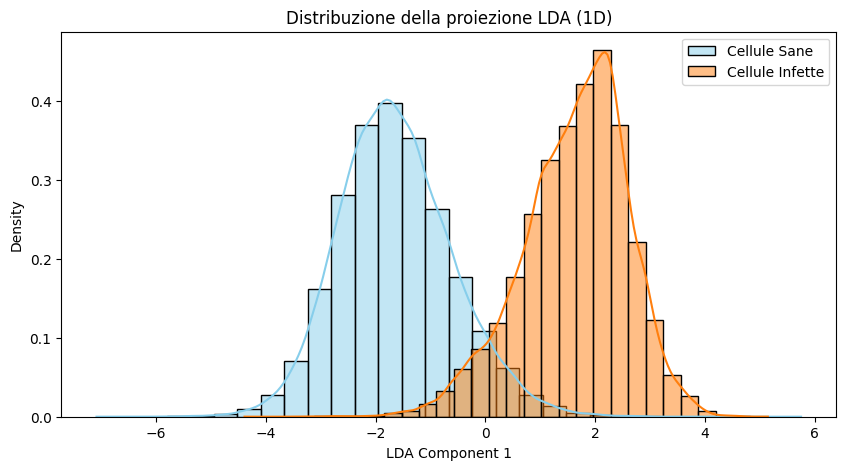
\includegraphics[width=.7\linewidth]{figures/lda_1.png}
  \caption{Distribuzione delle classi Cellule Sane e Cellule Infette.}
  \label{fig:lda_sano_infetto}
\end{figure}
%

Come mostrato in Figura~\ref{fig:lda_sano_infetto}, l’LDA consente di ottenere una buona separazione tra cellule sane e infette lungo una singola componente discriminante, facilitando il compito del classificatore.

\item \textbf{Secondo stadio – Classificazione delle cellule infette:} \\
Una volta identificate le cellule infette, esse vengono passate a un secondo classificatore, il cui obiettivo è quello di distinguere tra le sottoclassi patologiche: \texttt{trophozoite}, \texttt{ring}, \texttt{difficult}, \texttt{schizont} e \texttt{gametocyte}. In questo caso, il numero massimo di componenti LDA applicabili è $n_{classi} - 1 = 5$. È stata quindi eseguita un’ulteriore riduzione dimensionale tramite LDA, al fine di valutare la separabilità delle classi anche in questo sottoinsieme.


% 
\begin{figure}[H]
  \centering
  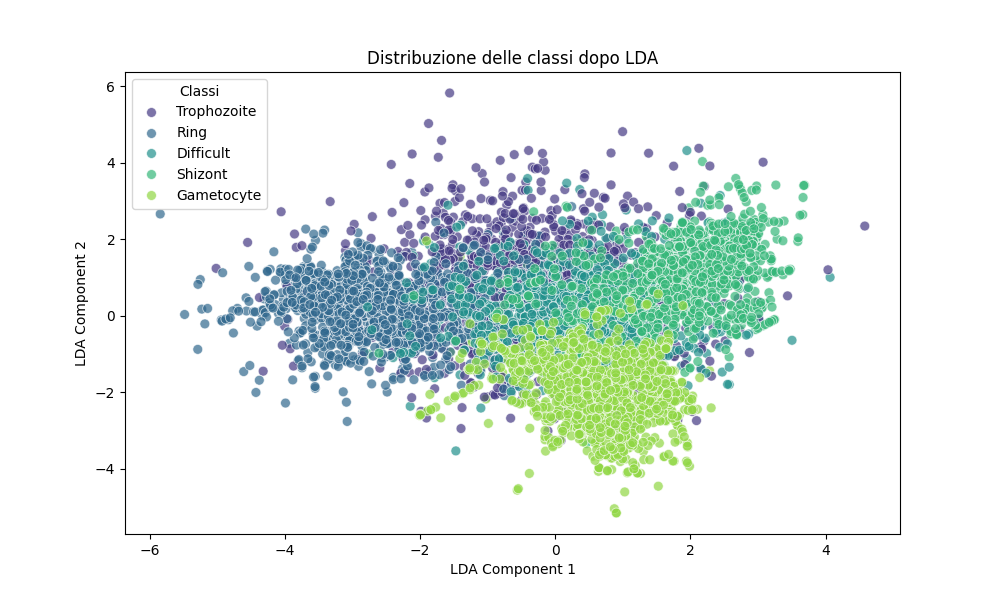
\includegraphics[width=.8\linewidth]{figures/lda_distribution.png}
  \caption{Distribuzione delle classi delle Cellule Infette.}
  \label{fig:lda_infette}
\end{figure}
%

Come evidenziato dalla Figura~\ref{fig:lda_infette}, la separabilità tra alcune classi migliora (si distinguono bene i globuli bianchi) mentre altre classi infette presentano una parziale sovrapposizione. Questo supporta l’efficacia dell’approccio gerarchico, in quanto la prima distinzione grossolana permette di alleggerire il carico del secondo classificatore, migliorando la performance complessiva del sistema.

\end{itemize}

\Section{Model training}
Sono stati valutati diversi modelli di classificazione, tra cui:

Possiamo fare o una tabella oppure un diagramma del genere



\begin{itemize}
\item \textbf{Non parametrici}: K-Nearest Neighbors (KNN)
\item \textbf{Lineari}: Logistic Regression
\item \textbf{Support Vector Machine (SVM)}: SVM con kernel lineare e non lineare (?)  
\item \textbf{Classificatori d’insieme}: Random Forest, XGBoost
\end{itemize}

dove:

\begin{itemize}

\item \textbf{K-Nearest Neighbors (KNN)}: È un algoritmo non parametrico basato sulla distanza. Per classificare un'istanza, considera i kkk esempi più vicini (in genere in termini di distanza euclidea) e assegna la classe più rappresentata tra questi. KNN non assume alcuna forma funzionale dei dati e può adattarsi bene a problemi non lineari, ma può essere sensibile alla scelta di kkk e alle caratteristiche dei dati (come la scala delle feature).

\item \textbf{Logistic Regression}: È un modello lineare di classificazione che stima la probabilità che un'osservazione appartenga a una certa classe utilizzando la funzione logistica (sigmoide). È semplice, interpretabile ed efficace quando le classi sono linearmente separabili, ma può avere prestazioni limitate su problemi complessi e non lineari.

\item \textbf{Support Vector Machine (SVM)}: L'SVM cerca l'iperpiano che massimizza il margine tra le classi. Grazie all'uso del kernel trick, può proiettare i dati in spazi di dimensioni superiori, permettendo la separazione anche in casi non linearmente separabili. È efficace in spazi ad alta dimensionalità ma può richiedere una buona scelta di iperparametri (come CCC e il tipo di kernel).

\item \textbf{Random Forest}: È un metodo ensemble basato su una collezione di alberi decisionali addestrati su diversi sottocampioni del dataset. La classificazione viene effettuata tramite voto di maggioranza. È robusto, gestisce bene l'overfitting e può modellare relazioni complesse, ma tende ad essere meno interpretabile.

\item \textbf{XGBoost (Extreme Gradient Boosting)}: È un potente algoritmo di boosting che costruisce alberi in sequenza, dove ciascun nuovo albero corregge gli errori dei precedenti. Ottimizza una funzione di perdita tramite gradient boosting ed è noto per la sua alta accuratezza e efficienza computazionale. Tuttavia, richiede una maggiore attenzione nell’ottimizzazione degli iperparametri per evitare overfitting.

\end{itemize}

L'ottimizzazione degli iperparametri è stata effettuata mediante \texttt{RandomizedSearchCV}, con una validazione incrociata a 3 fold e ottimizzazione rispetto all'\textbf{F1 score macro}, al fine di tenere conto dell'eventuale sbilanciamento tra le classi.


\Section{Model evaluation}

Al termine della fase di addestramento, la miglior configurazione degli iper-parametri trovata utilizzando \texttt{RandomizedSearchCV} è \hlight{SVM} con :
\ifshowcode
%
\begin{code}{python}
  param_dist = {
        'selector__k': [700],
        'classifier__C': [100],
        'classifier__kernel': ['poly'],
        'classifier__gamma': ['auto'] 
    }
\end{code}
%
\fi
La valutazione delle performance del modello finale è stata effettuata confrontando le predizioni sul test set con le etichette reali, utilizzando le seguenti metriche:

\begin{itemize}
\item \textbf{Balanced Accuracy}: particolarmente utile in presenza di classi sbilanciate.
\item \textbf{F1-Score Macro}: media armonica tra precision e recall, calcolata su tutte le classi, trattandole equamente.
\item \textbf{Precision e Recall per classe}, per una valutazione più granulare delle performance.
\item \textbf{Matrice di confusione}, per visualizzare gli errori di classificazione tra le diverse classi.
\end{itemize}

Tutte le metriche e i risultati sono stati salvati automaticamente in un file di log, per garantire la tracciabilità e la riproducibilità degli esperimenti.

% 
\begin{figure}[H]
  \centering
  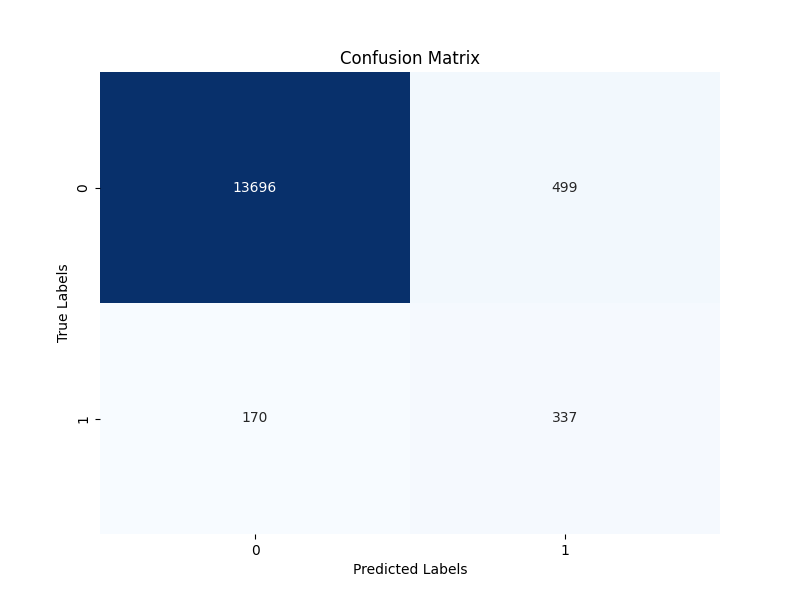
\includegraphics[width=.8\linewidth]{figures/confusion_matrix_Stage 1 - SVM.png}
  \caption{Matrice di Confusione del primo Classificatore.}
  \label{fig:confusion_1}
\end{figure}
% 
\begin{figure}[H]
  \centering
  \includegraphics[width=.8\linewidth]{figures/confusion_matrix_Stage 2 - SVM ➡ SVM.png}
  \caption{Matrice di Confusione del secondo Classificatore.}
  \label{fig:confusion_2}
\end{figure}
%









\iffalse

\Section{Title Formatting}
To begin a new content, always start the content with a chapter heading. To
insert the chapter with an additional \lstinline[columns=fixed]{minitoc}
use \lstinline[columns=fixed]{\Chapter}, which produces an heading as
you see at the beginning of this page, to have a heading without
a \lstinline[columns=fixed]{minitoc} use the standard
\lstinline[columns=fixed]{\chapter}.

The document relies on the user to use the \hlight{correct} title commands to
keep the formatting consistent. The commands that starting with a
capital letter are the overloaded commands of the standard ones.
The following are the current ones:
%
\begin{code}{python}
\Chapter{...}
\Section{...}
\Subsection{...}
\Subsubsection{...}
\end{code}
%
\begin{warning}
	Unless there is a specific reason, it is suggested to use the aforementioned
	commands. However, original LaTeX command should work as well if you want to use.
\end{warning}

\Subsection{Page Geometry}

The page geometry is set to the following settings. This is done using the
standard package \pcode{\usepackage{geometry}} which is defined in the
\pcode{Hebdomon.cls}.
%
\begin{itemize}[leftmargin=!,labelindent=-29.2pt]
	\item[\textbf{top}] 2.5cm,
	\item[\textbf{right}] 2.0cm,
	\item[\textbf{bottom}] 2.5cm,
	\item[\textbf{left}] 3.0cm.
\end{itemize}
%
\Section{Image Positioning}
%
The image positioning could be done with the following code snippet:
%
\begin{code}{latex}
\begin{figure}[ht]
  \centering
  \includegraphics[options]{figures/path.pdf}
  \caption{\label{fig:label} }
\end{figure}
\end{code}
%
Here there are a few options worth mentioning:
%
\begin{hgitemize}
	\item[\pcode{figures/path}] The place where the image is kept. If the
	image is in the same folder where the main.tex file resides, it is as
	simple as writing the files name. If the file is in a folder called
	image, just write \pcode{image/innsbruck.jpg}. Finally if the image is
	in a higher directory (i.e., image is in folderA/innsbruck.jpg and the
	main tex is in folderA/document/main.tex then the path becomes \pcode{../innsbruck.jpg}
	\item[\pcode{\caption{..}}] Where you write the caption of the image.
	For consistency make sure every image has a caption as if the image does not
	need a caption, maybe it not be present to begin with.
	\item[\pcode{label{}}] This is an identifier for you to use when you need
	to cite this Figure in a place somewhere. For example if you were to have
	and image with the following:
\end{hgitemize}
%
\begin{code}{latex}
\begin{figure}[ht]
  \centering
  \includegraphics[width=\textwidth]{figures/path.pdf}
  \caption{A photo I found on the web.}\label{fig:innsbruck}
\end{figure}
\end{code}
%
\begin{hgitemize}
	\item[] Now this image is referenced as \pcode{fig:innsbruck}, which
	means if we write the following:
\end{hgitemize}
%
\begin{code}{text}
To see the image, have a look at Figure \ref{fig:innsbruck}
\end{code}
%
This line of command will be presented as
%
\begin{excerpt}
	To see the image, have a look at Figure 1.1.
\end{excerpt}
%
Finally you can see the image here as well.
%
\begin{figure}[ht]
	\centering
	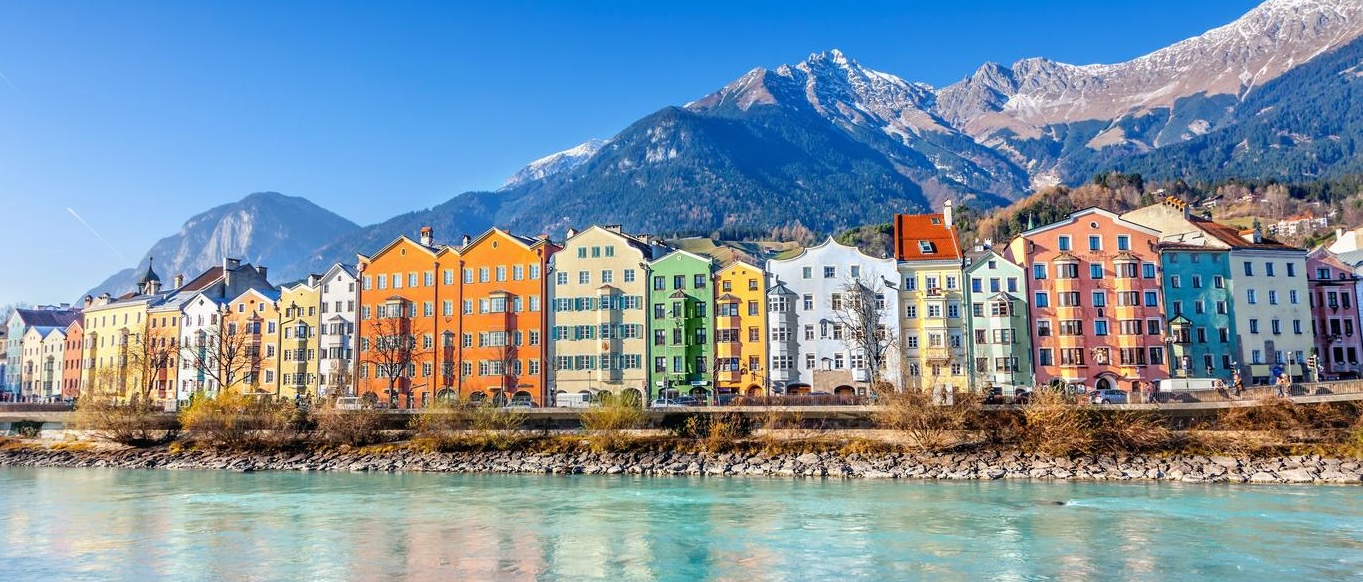
\includegraphics[width=\linewidth]{figures/innsbruck.jpg}
	\caption{The famous Innsbruck houses near the river Inn. This image is
		placed with a width value of \pcode{width=\linewidth}. This is also
		a good opportunity to showcase the hanging behaviour of the figure
		caption.}
\end{figure}
%
\Section{Defined Environments}
%
\begin{hgitemize}
	\item[\pcode{excerpt}] The template relies on the excellent \lstinline[columns=fixed]{tcolorbox}
	package for formatting the boxes within the document and for that end different styles were created.
	\item[] Sometimes one needs to quote either a proverb or to create drama, for this use
	the \lstinline[columns=fixed]{excerpt} environment with the following notation and effect.
\end{hgitemize}
%
\begin{code}{latex}
\begin{excerpt}
  To be, or not to be...
\end{excerpt}
\end{code}
%
\begin{hgitemize}
	\item[] Compiling this code snippet would show as in the document
\end{hgitemize}
%
\begin{excerpt}
	To be, or not to be...
\end{excerpt}
%
\begin{itemize}[leftmargin=!,labelindent=-29.2pt]
	\item[\pcode{code}] During the preparation of your document, it is useful to showcase
	      some code either in the shape of all the document or a snippet of it.
	      There are two (\hlight{2}) ways of doing this where the first one will be discussed here.
	\item[] For example to print out a hello world in python, please use the following environment
\end{itemize}
%
\begin{verbatim}
\begin{code}{python}
print("Hello, World!")
\end{code}
\end{verbatim}
%
Producing the following:
%
\begin{code}{python}
print("Hello, World!")
\end{code}
%
The class also come with some predefined environments to modify the behaviour/aesthetics of the document.
%
Highlighting text is \hlight{very easy}, here is an example on how to write one.

\begin{code}{latex}
Highlighting text is \hlight{very easy}, here is an example:
\end{code}

\begin{itemize}[leftmargin=!,labelindent=-29.2pt]
	\item[\pcode{example}] Sometimes you need to showcase an example or
	      need to highlight a certain idea.
	      For these things the environment Example could be useful.
	\item[] For example to show as simple example or give a slight attention to a topic you can do the following.
\end{itemize}

\begin{example}
	This is an example. This could be anything which you would like to have a certain amount of
	attention but not too much as to distract from the flow of the document.
\end{example}

\begin{itemize}[leftmargin=!,labelindent=-29.2pt]
	\item[\pcode{highlight}] Or sometimes you need to give a clear break to the flow of the
	      document and ask the reader to look at your banner. For that use highlight.
\end{itemize}

\begin{highlight}
	Hey! Pay attention as this is a highlight box.
\end{highlight}

\Subsection{Writing Equations}
%
One of the strong suits of LaTeX compared to other editors and programs is
it simplicity and ease of use methods of writing equations. Consider the
following equation:
%
\begin{equation*}
	f(x) = x^2 + 2x + 1
\end{equation*}
%
In code form this would be written as:
%
\begin{code}{latex}
	\begin{equation*}
		f(x) = x^2 + 2x + 1
	\end{equation*}
\end{code}
%
All equations that has their newline and centre staged are mostly written
in an environment where it has a \pcode{begin} and an \pcode{end}. You may
have noticed the asterisks sign just after the equation. This implies the
environment is \hlight{not numbered}, meaning you won't be able to
reference it. This is used to limit the numbering of equations to just the
essential parts in the document and not reach 3 digits by the time you are
in page 8. For a numbered equation like the following
%
\begin{equation}
	f(x) = x^2 + 2x + 1
\end{equation}
%
You only need to do:
%
\begin{code}{latex}
	\begin{equation}\label{eq:quad}
		f(x) = x^2 + 2x + 1
	\end{equation}
\end{code}
% 
where \pcode{\label{eq:quad}} is the equation reference label.
%
You could also make matrices as well as \pcode{amsmath} is preloaded into this template.
%
\Subsection{Designing a Table}
%
Finally, no template is done without someone telling you how a table should be designed.
%
Below is a standard table
%
\begin{table}[!ht]
	\begin{NiceTabular}{rX}[rules/color=[gray]{0.9},rules/width=1pt]
		\CodeBefore
		\rowcolors{1}{black!5}{}
		\rowcolors{3}{blue!5}{}
		\Body
		\toprule
		\textbf{Section}      & \textbf{Scientific Method Step}                                \\
		\midrule
		\textbf{Introduction} & states your hypothesis                                         \\
		\textbf{Methods}      & details how you tested your hypothesis                         \\
		\textbf{Results}      & provides raw (i.e., uninterpreted) data collected              \\
		\textbf{Discussion}   & considers whether the data you obtained support the hypothesis \\
		\bottomrule
	\end{NiceTabular}
	\caption{A Detailed look into the scientific method.}
\end{table}
%
And the code used to generate it:
%
\begin{code}{latex}
\begin{table}[!ht]
	\begin{NiceTabular}{rX}[rules/color=[gray]{0.9},rules/width=1pt]
		\CodeBefore
		\rowcolors{1}{black!5}{}
		\rowcolors{3}{blue!5}{}
		\Body
		\toprule
		\textbf{Section}      & \textbf{Scientific Method Step}    \\
		\midrule
		\textbf{Introduction} & states   hypothesis                \\
		\textbf{Methods}      & how you tested hypothesis          \\
		\textbf{Results}      & provides raw  data collected       \\
		\textbf{Discussion}   &  whether it support the hypothesis \\
		\bottomrule
	\end{NiceTabular}
	\caption{A Detailed look into the scientific method.}
\end{table}
\end{code}

\Chapter{Plotting your data using PGF/TikZ}

\Section{Introduction}

PGFplots and Tikz are powerful scripting languages allowing you to draw high-quality diagrams
using only a programming language. PGFplots are generally used for plotting data from a wide
variety of representations from simple 2D plots to complex 3D geometries.
\\
But wikipedia description put it best:

\begin{excerpt}
	PGF/TikZ is a pair of languages for producing vector graphics
	(e.g., technical illustrations and drawings) from a geometric/algebraic description, with
	standard features including the drawing of points, lines, arrows, paths, circles,
	ellipses and polygons. PGF is a lower-level language, while TikZ is a set of higher-level
	macros that use PGF. The top-level PGF and TikZ commands are invoked as TeX macros,
	but in contrast with PSTricks, the PGF/TikZ graphics themselves are described in a
	language that resembles MetaPost.
\end{excerpt}

For more info please look at the documentation \href{https://tikz.dev/pgfplots/}{here}.
It is of course up to the user to select which graphical software to produce the necessary
visual components but unless it requires complex functions/processing, it would be be easier
to have it in PGF/TikZ format for easy editing/maintenance.

For this manual we will be looking at the three (\hlight{3}) plot types you may
encounter in your studies.
%
\Subsection{A Simple 2D Plot}
%
2D plots are simple yet powerful to show the relation of a single parameters
and its related function.
Below is an example of a simple comparison of two (\hlight{2}) functions.
%
\begin{figure}[!ht]
	\centering
	\begin{tikzpicture}
		\begin{axis}[hebdomon, xlabel = \(x\), ylabel = {\(f(x)\)}]
			% 
			\addplot [domain=-10:10, samples=100,red]{x^3 - 7*x - 1};
			\addlegendentry{\(x^2 - 2x - 1\)}
			%
			\addplot [domain=-10:10, samples=100, blue]{x^2 + 6*x + 8};
			%
			\addlegendentry{\(x^2 + 2x + 1\)}
			%
		\end{axis}
	\end{tikzpicture}
	\caption{This is an example of a 2D PGF plot comparing
		two functions where these functions are calculated using
		PGF itself rather than entering/reading from data.}
\end{figure}
%
The image above is generated using the following code:

\begin{code}{latex}
\begin{figure}[!ht]
  \centering
  \begin{tikzpicture}
    \begin{axis}[hebdomon, xlabel = \(x\), ylabel = {\(f(x)\)}]
      % 
      \addplot [domain=-10:10, samples=100,red]{x^3 - 7*x - 1};
      \addlegendentry{\(x^2 - 2x - 1\)}
      % 
      \addplot [domain=-10:10, samples=100, blue]{x^2 + 6*x + 8};
      % 
      \addlegendentry{\(x^2 + 2x + 1\)}
      % 
    \end{axis}
  \end{tikzpicture}
  \caption{This is an example of a 2D PGF plot comparing
  two functions where these functions are calculated using
  PGF itself rather than entering/reading from data.}
\end{figure}
\end{code}

As can be seen it is relatively standard to create plots. Some aspect
which need mentioning.

\begin{hgitemize}
	\item[\pcode{\addplot}] You invoke this command when you want to
	create a plot. In the square brackets (i.e., []) you insert your
	\hlight{configuration} of your plot. The most important ones are
	\begin{itemize}
		\item[\pcode{domain}] the range in which the function will be
		      calculated
		\item[\pcode{sample}] the number of calculations will be done
		      within the defined domain.
	\end{itemize}
\end{hgitemize}

\Subsection{Plotting 3D plots}

Plotting data with PGFplots is also quite possible and will generate
great plot (as long as it is not massively complicated). For more
information on the precautions on designing 3D plots, please have a look
at \href{https://tikz.dev/pgfplots/reference-3dplots}{here}.

Below is the prototypical plot to showcase the 3D capabilities of PGF:

\begin{figure}[!ht]
	\centering
	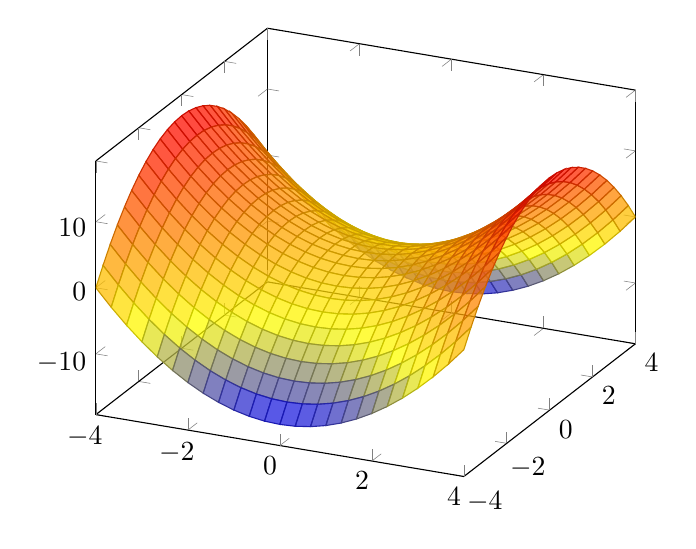
\begin{tikzpicture}
		\begin{axis}[view={25}{30},mark layer=like plot]
			\addplot3 [
				surf,
				shader=faceted,
				fill opacity=0.75,
				samples=25,
				domain=-4:4,
				y domain=-4:4,
				on layer=main,
			] {x^2-y^2};
		\end{axis}
	\end{tikzpicture}
	\caption{An example 3D plot done wit PGFplots.}
\end{figure}

And, of course the code for generating the plot is given as follows:

\begin{code}{latex}
\begin{figure}[!ht]
  \centering
  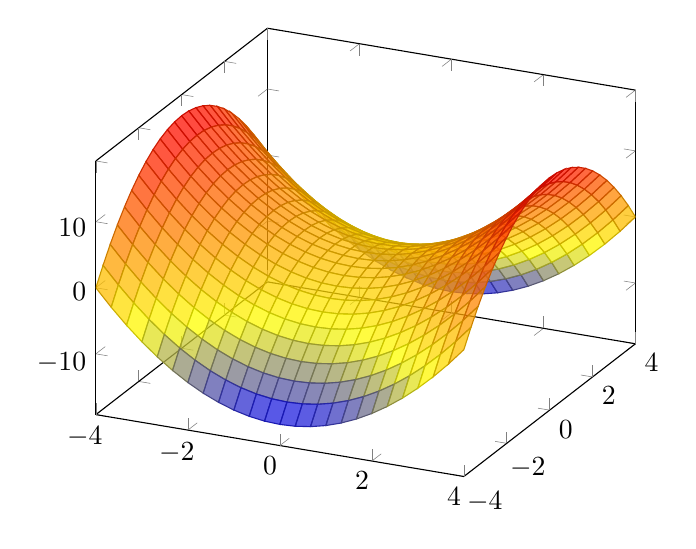
\begin{tikzpicture}
    \begin{axis}[view={25}{30},mark layer=like plot]
      \addplot3 [
      surf,
      shader=faceted,
      fill opacity=0.75,
      samples=25,
      domain=-4:4,
      y domain=-4:4,
      on layer=main,
      ] {x^2-y^2};
    \end{axis}
  \end{tikzpicture}
  \caption{An example 3D plot done wit PGFplots.}
\end{figure}
\end{code}

Some options worth mentioning are as follows:

\begin{hgitemize}
	\item[\pcode{surf}] Generates a \hlight{surface} based on the 2D
	data it was given (in this case these are $x$ and $y$.
	\item[\pcode{shader}] Describes, basically how each segment should be
	filled.
	\item[\pcode{samples}] Similar to 2D plots, tells how many data points will
	be measured. However, make a note that 3D is significantly more taxing
	on the TeX memory than 2D and making this sampling high may result in
	exceeding the memory limit.
\end{hgitemize}


\fi


\end{document}

%%% Local Variables:
%%% coding: utf-8
%%% mode: latex
%%% TeX-command-extra-options: "-shell-escape"
%%% TeX-master: t
%%% TeX-engine: luatex
%%% End:

